\subsection{Method Overview}

% This section details the methods researched for modeling historical map point observability, and explores how it may be used to identify outdated map points. The methods explored here will be tested and benchmarked in Section \ref{sec:analysis} to determine if the objectives laid out in Section \ref{sec:objectives} are successfully achieved.

% The objective is to identify map points which, while previously viewed, are no longer visible due to environmental changes. To address this, we assign an incrementally updated probability of existence value to each map point. Observations of a map point increase our overall confidence in its existence. Conversely, failure to observe a map point from a viewpoint where it \textit{should} have been visible lowers our confidence in its existence. Determining whether a map point should be observable from a given viewpoint is not trivial, motivating the need for a viewpoint-aware observability model. The purpose of the model is to integrate historical observability data to estimate observability across all possible viewpoints. Each map point is attached to its own model.

\subsubsection{The Existence Estimation Framework}

The proposed existence estimation framework iteratively updates the existence probability for a KV-SLAM map point using historical observability priors and current observations. As shown in Figure \ref{fig:existence_estimation_framework}, the framework consumes new observational data, and outputs an updated estimate of the point's probability of existence.

\begin{figure}[!ht]
    \centering
    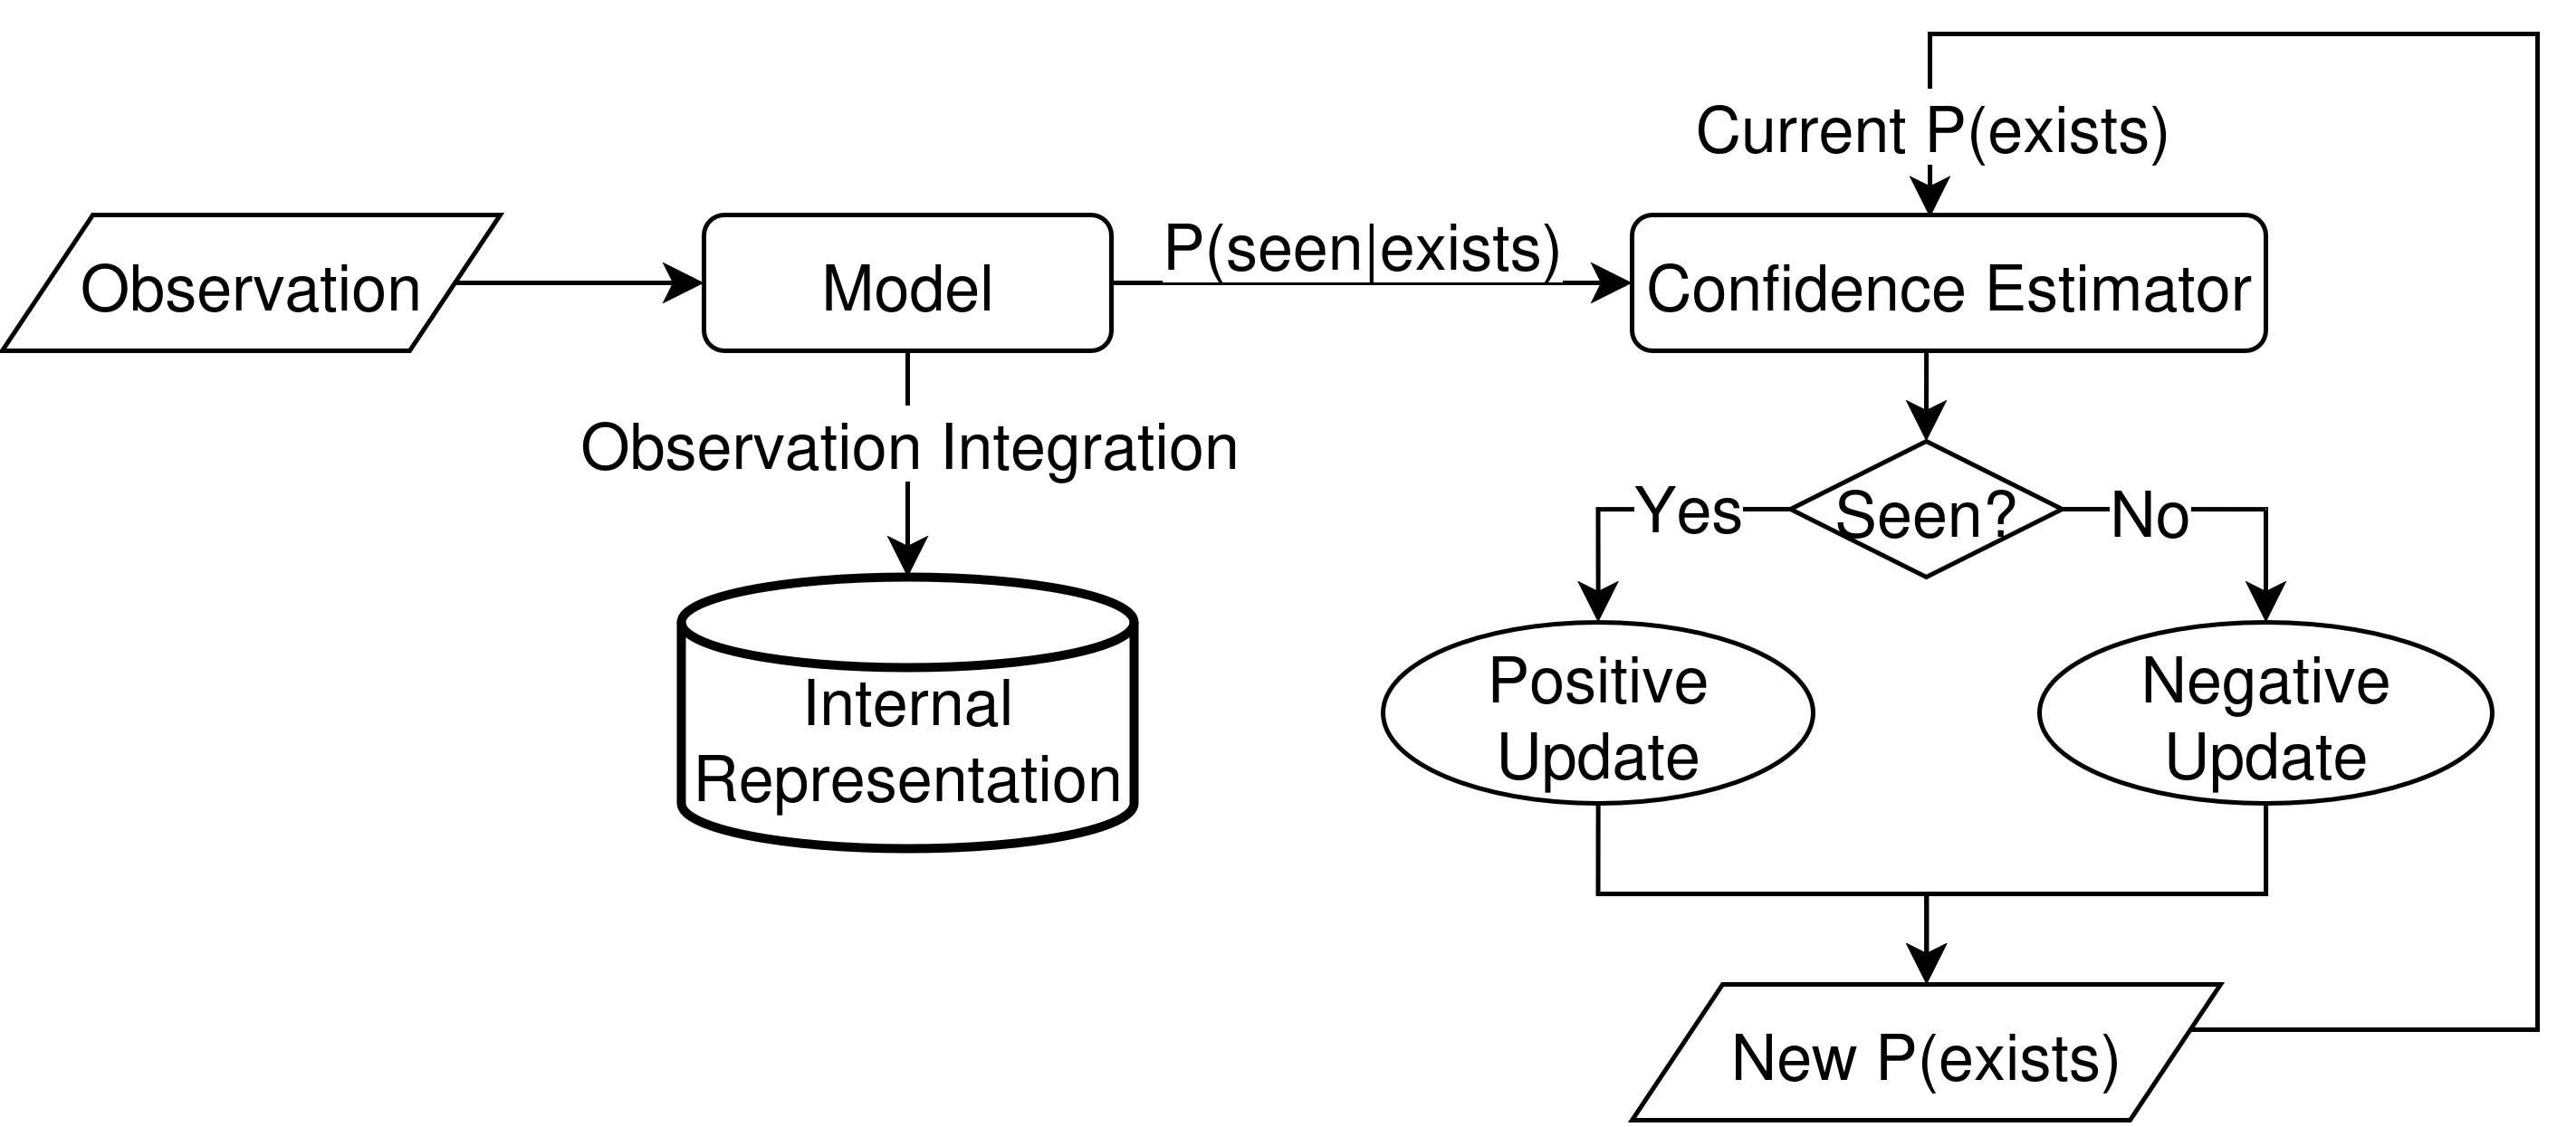
\includegraphics[width=0.7\textwidth]{resources/existence_estimation_framework.png}
    \caption[Existence Estimation Framework]{A flowchart representing the flow of data through the proposed Existence Estimation Framework.}
    \label{fig:existence_estimation_framework}
\end{figure}

The framework consists of two components: the observability model, and the existence probability updater. The observability model estimates the probability of a point being seen from a given viewpoint $P(S^{\boldsymbol{v}}|E)$, and updates its internal representation to integrate new observations. The existence probability updater performs a Bayesian update of the point's existence probability using the prior existence probability $P(E)$, the model estimate $P(S^{\boldsymbol{v}}|E)$, and the new observation's outcome $S$ or $\lnot S$. This approach ensures that negative observations from previously highly observable viewpoints impact the existence probability more strongly than those from more uncertain viewpoints.

\subsubsection{The Bayesian Update Step}

The system updates its confidence for a map point's existence based on environmental observations. This update follows Bayes' theorem, and can therefore be implemented to utilize Bayesian statistics. The events of interest are:
\begin{itemize}
    \item $E$: The event that the map point exists
    \item $S^{\boldsymbol{v}}$: The event that the map point is seen from viewpoint $\boldsymbol{v}$
\end{itemize}

where $\boldsymbol{v} = \{\theta,\phi,d\}$, representing azimuth, elevation and distance from the observer to the point respectively. To formalize, our system updates $P(E) = P(E|S^{\boldsymbol{v}})$ given a positive observation, and $P(E) = P(E|\neg S^{\boldsymbol{v}})$ given a negative observation.

Applying Bayes' theorem, the derived update function is
\[
    P(E) = \begin{cases}
        \frac{P(S^{\boldsymbol{v}}|E)P(E)}{P(S^{\boldsymbol{v}})}           & \text{given }S^{\boldsymbol{v}}      \\
        \frac{P(\neg S^{\boldsymbol{v}}|E)P(E)}{P(\neg S^{\boldsymbol{v}})} & \text{given }\neg S^{\boldsymbol{v}}
    \end{cases}
\]

Additionally, the marginal probability $P(S^{\boldsymbol{v}})$ is
$$
    P(S^{\boldsymbol{v}}) = P(S^{\boldsymbol{v}}|E)P(E) + P(S^{\boldsymbol{v}}|\neg E)P(\neg E)
$$

The probability of a false observation of a non-existent map point is small, but non-zero. The probability of a false match increases in low-light and in low texture environments. The value $\varepsilon$ is assigned to represent this probability, and will be experimentally determined in Section \ref{sec:existence_confidence_eval}.
$$
    \varepsilon = P(S^{\boldsymbol{v}}|\neg E) \approx 0
$$

Finally, assuming the existence of a model function $m$ which estimates the probability of observing the point from a given viewpoint $\boldsymbol{v}$
$$
    m(\boldsymbol{v}) \approx P(S^{\boldsymbol{v}}|E)
$$

The update step can be expressed as
\[
    P(E) = \begin{cases}
        \frac{m(\boldsymbol{v})P(E)}{m(\boldsymbol{v})P(E) + \varepsilon(1-P(E))}             & \text{given }S^{\boldsymbol{v}}      \\
        \frac{(1-m(\boldsymbol{v}))P(E)}{(1-m(\boldsymbol{v}))P(E) + (1-\varepsilon)(1-P(E))} & \text{given }\neg S^{\boldsymbol{v}}
    \end{cases}
\]

\subsubsection{The Observability of Map Points}

Map points are conceptualized as static, infinitesimally small points in 3D Euclidean space. Let the observability of a map point $p$ from a viewpoint $\boldsymbol{v} = \{\theta,\phi,d\}\in[0,2\pi)\times\left[-\frac{\pi}{2},\frac{\pi}{2}\right]\times[0,d_{max})$ be represented by the function
$$
    \operatorname{observable}_p : V \to \{0, 1\}
$$
where $\boldsymbol{v} = \{\theta,\phi,d\}$ represents the azimuth, elevation, and distance from the observer to $p$ respectively. This function returns 1 if $p$ is observed from $\boldsymbol{v}$, and 0 if it is not. From this, an observation of point $p$ can be defined as a vector $\boldsymbol{o}_p=\{\boldsymbol{v},observable_p(\boldsymbol{v})\}$, and a set of $n$ observations of $p$ as $\boldsymbol{O}_p=\{\boldsymbol{o}_{p0},\dots,\boldsymbol{o}_{pn}\}$. For illustrative purposes, figures in the remainder of this thesis may use a simplified 2D representation of these definitions, where $\boldsymbol{v}^{2D}=\{\theta,d\}$. Figure \ref{fig:global_observability_p} shows such a plot representing the global observability of a map point $p$, and the effects of obstructions on observability.

\begin{figure}[!ht]
    \centering
    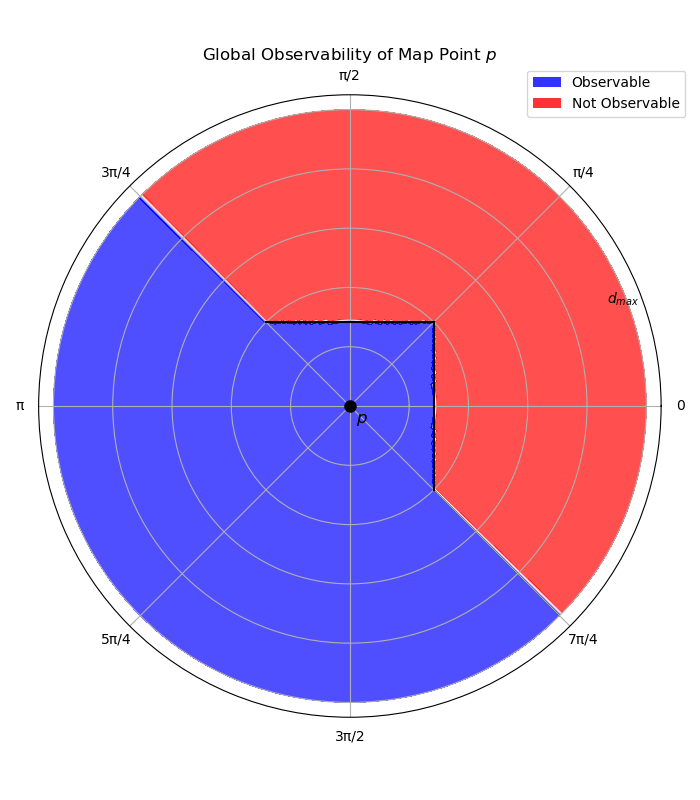
\includegraphics[width=0.7\textwidth]{resources/global_observability_p.png}
    \caption[2D Global Observability]{A 2D representation of the global observability of a map point $p$ near two orthogonal obstructions.}
    \label{fig:global_observability_p}
\end{figure}

The generation of such a plot would require the generation and storage of infinite observations across the 

\subsubsection{Modeling Historical Observability of Map Points}

The goal of the model is to estimate the global observability of a point using a finite set of $n$ observations $\boldsymbol{O} = \{o_0,\dots,o_n\}$, an implementation-dependent set of $k$ model parameters $\boldsymbol{x}=\{x_0,\dots,x_k\}$, and a current viewpoint $\boldsymbol{v}$.
$$
    m(\boldsymbol{O},\boldsymbol{x},\boldsymbol{v})\to[0,1]
$$

Therefore, the model functions will be implemented with the goal of minimizing the objective function
$$
    \iiint |m(\boldsymbol{O},\boldsymbol{x},\boldsymbol{v}) - v(\boldsymbol{v})| \,d\theta\,d\phi\,dd
$$

Additionally, the models are constrained by the goals laid out in Section \ref{sec:objectives} for speed and size of the model. The integrated version which will be described in Section \ref{sec:orb_slam3_integration} must run in real time, meaning inserting new observations should be fast. Additionally, as the model parameters will be stored in memory during operations, and written to disk for map reuse, the additional space required by the model must be minimized. Each of the three models described will be compared for speed, size, and accuracy, and the parameters to each model will be tuned using non-linear optimization to determine the best possible parameterization. With these goals in mind, the model implementations can now be described. These models were selected based on their ease of implementation and simple methodology. This is not the complete set of possible implementations, and are not guaranteed to be the optimal solution to modeling historical map point observability while maximizing accuracy and minimizing time and storage usage.

\paragraph{K-Nearest Neighbors Model}
A simple method for modeling the observability is the use of a K-nearest-neighbors clustering method. The only parameter in such a model. Such a model could be formulated as follows:
$$
    m_{knn}(k, n, \boldsymbol{v}) = \frac{a}{b}
$$
\paragraph{Binned Model}
\paragraph{Continuous Model}